\chapter{Approximations of VIX options}

% In this section, we use the methods illustrated before to price options under several volatility models. In section \ref{sec: 3.1}, we approximate option prices with 1-dimensional volatility processes; In section \ref{sec: 3.2}, method is given to price options under double CEV model. In section \ref{sec: 3.3}, while pricing path-dependent options like American options, we use the DOI estimator and shows that it's able reduce simulations' variance.

\section{Approximating options under mean-reverting CEV model}
\label{sec: 3.1}

\subsection{Drawbacks of using Black-Scholes model as an auxiliary model}
\cite{chan_empirical_1992} proposes the mean-reversion CEV model, in which volatility follows

$$
    d V_{t}=\left(\alpha+\beta V_{t}\right) d t+\sigma V_{t}^{\gamma} d W_{t}
$$

\noindent when $\beta$ is negative, this model has mean-reverting property. We can rewrite it to be

\begin{equation}\label{mr}
    d V_t=\kappa(m - V_t) d t+\sigma V^{\gamma}_t d W_t
\end{equation}

\noindent where $\kappa$ is the speed of mean-reversion, $m$ is the long-run mean. A natural idea is to use Black-Scholes model as auxiliary model as mentioned in \cite{kristensen_adding_2011}, then apply their method to approximate the VIX option price under mean-reverting CEV model. Denote $\mathcal{L}$ and $\mathcal{L}^{\text{BS}}$ to be infinitesimal generators of mean-reverting CEV model and Black-Scholes model respectively

$$
\begin{aligned}
    \mathcal{L} w&= \frac{\partial w}{\partial t}+\kappa(m - V) \frac{\partial w}{\partial V}+\frac{1}{2} \sigma^{2} V^{2\gamma} \frac{\partial^{2} w}{\partial V^{2}} \\
    \mathcal{L}^{\text{BS}} w &= \frac{\partial w}{\partial t}+rV \frac{\partial w}{\partial V}+\frac{1}{2} \sigma^{2} V^2 \frac{\partial^{2} w}{\partial V^{2}}
\end{aligned}
$$

\noindent The mis-pricing term for using Black-Scholes model is then

$$\delta^{\text{BS}} = (\mathcal{L} - \mathcal{L}^{\text{BS}}) w^{\text{BS}} = (\kappa - r)V \frac{\partial w^{\text{BS}}}{\partial t} + \kappa m \frac{\partial w^{\text{BS}}}{\partial t} + \sigma^{2} (V - V^{2 \gamma}) \frac{\partial^{2} w^{\text{BS}}}{\partial V^{2}} $$

\noindent with the solution of Black-Scholes model $w^{\text{BS}}$. Note that $\delta^{\text{BS}}$ contains theta and gamma of option. Their differences in Black-Scholes model and mean-reverting model determines that we have to use other auxiliary models.

Take call option prices under $\gamma=\frac{1}{2}$ in model\eqref{mr} as an example. This model is known as mean square root mean-reverting model proposed by \cite{grunbichler_valuing_1996}.


\begin{figure}[ht]
    \centering
    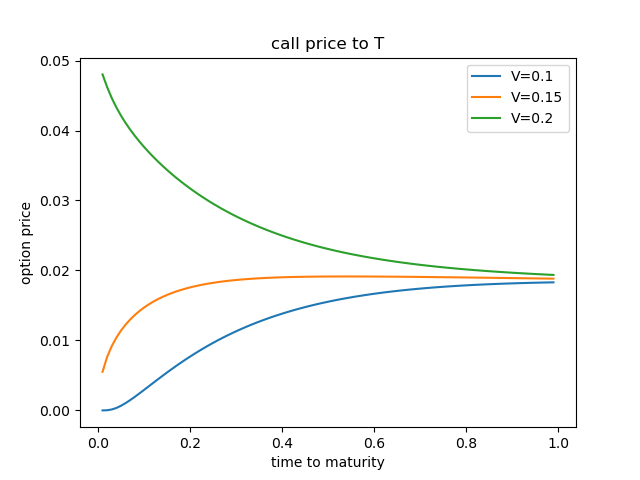
\includegraphics[width=10cm]{./figures/call2T.png}
    \caption{Call option price with regard to time to maturity}\label{call2t}
\end{figure}

\begin{figure}[ht]
    \centering
    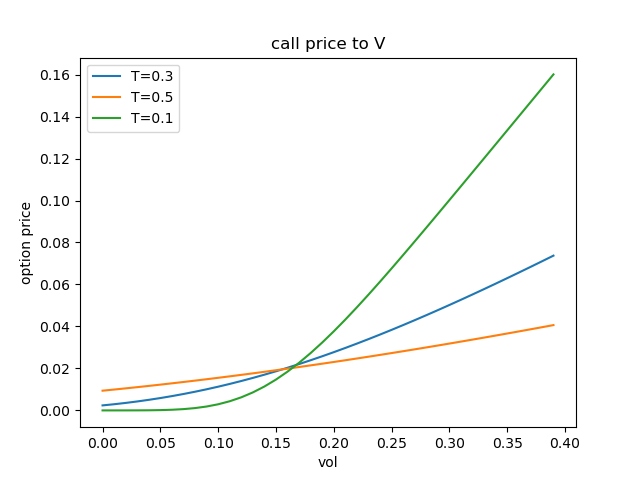
\includegraphics[width=10cm]{./figures/call2V.png}
    \caption{Call option price with regard to volatility}\label{call2v}
\end{figure}

From figure \ref{call2t}, we can find that in contrast to Black-Scholes model, the value of call option price under mean-reverting model is not always increasing as time to maturity increases; From figure \ref{call2v}, by contrast, the call option price does not converge to zero as volatility goes to zero. In addition, \cite{grunbichler_valuing_1996} also shows that $V$ has less influence of the current value of the call option than in Black-Scholes model. For these reasons, we conclude that Black-Scholes model is not an appropriate auxiliary model and in the next section, we discuss that using the square root mean-reverting model as the auxiliary model.

\subsection{Using square root mean-reverting model as auxiliary model}

Recall the mean-reverting CEV model with $\gamma=\frac{1}{2}$

\begin{equation}
    d V_t=\kappa(m - V_t) d t+\sigma \sqrt{V_t} d W_t
\end{equation}

We are going to use it as our auxiliary model as it captures the mean-reverting property of general mean-reverting CEV models. \cite{grunbichler_valuing_1996} gives an explicit solution to this model. Denote the call option price $\bar{w}$ with strike $K$, constant risk-free rate $r$, time to maturity $T$ and no expected premium for volatility risk is paid, its price is given by

\begin{equation}\label{aux call price}
    \begin{aligned}
        \bar{w}=&  e^{ -(\kappa+r) T} V Q(x K ; \nu+4, \lambda) \\
        &+ m e^{-r T}(1-e^{-\kappa T}) Q(xK ; \nu+2, \lambda) \\
        &-e^{-r T} K Q(x K; \nu, \lambda)
        \end{aligned}
\end{equation}

\noindent where

$$
\begin{aligned}
    &x=\frac{4 \kappa}{\sigma^{2}(1-e^{-\kappa T})} \\
    &\nu=\frac{4 \kappa m}{\sigma^{2}}, \\
    &\lambda= e^{-\kappa T}x V
    \end{aligned}
$$

\noindent and $Q(xK ; \nu+i, \lambda)$ is the complementary distribution function for the non-central chi-squared density with $\nu + i$ degrees of freedom and non-centrality parameter $\lambda$.

Define the infinitesimal generators $\bar{\mathcal{L}}$ for square root mean-reverting model and $\mathcal{L}$ for mean-reverting CEV model

\begin{equation}\label{inf gen1}
    \begin{aligned}
        \mathcal{L} w&= \frac{\partial w}{\partial t}+\kappa(m - V) \frac{\partial w}{\partial V}+\frac{1}{2} \sigma^{2} V^{2\gamma} \frac{\partial^{2} w}{\partial V^{2}} \\
        \bar{\mathcal{L}} w &= \frac{\partial w}{\partial t}+\kappa(m - V) \frac{\partial w}{\partial V}+\frac{1}{2} \sigma^{2} V \frac{\partial^{2} w}{\partial V^{2}}
    \end{aligned}
\end{equation}

Subtract infinitesimal generators in equation\eqref{inf gen1}, we get the mis-pricing formula for using square root mean-reverting model

$$
\delta = (\mathcal{L} - \bar{\mathcal{L}}) \bar{w} = \frac{1}{2} \sigma^{2} (V^{2\gamma} - V) \frac{\partial^{2} w}{\partial V^{2}}
$$

\noindent We can then use the approximation formula discussed in \ref{sec: 2.2} to price call options under mean-reverting CEV model\footnote{Put options can be priced easily in the same way}

\begin{equation} \label{cev approx formula}
    w_{N}(t, x)=\bar{w}(t,x)+\sum_{n=0}^{N} \frac{(T-t)^{n+1}}{(n+1) !} \delta_{n}(t, x)
\end{equation}

\noindent where

\begin{equation}\label{mispricing}
    \begin{aligned}
        &\delta_0 = \delta = \frac{1}{2} \sigma^{2} (V^{2\gamma} - V) \frac{\partial^{2} w}{\partial V^{2}} \\
        &\delta_{n}(t, x)=L \delta_{n-1}(t, x)- r\delta_{n-1}(t, x)
        \end{aligned}
\end{equation}

Finally we get a closed form approximating formula for call options under mean-reverting CEV model. But notice that the call price \eqref{aux call price} contains non-square chi square distribution functions, applying infinitesimal generator $\mathcal{L}$ on it can be a hard point and in the next section we are going to talk about how to derive partial derivatives of distribution function $Q(\cdot | \nu+i, \lambda)$.

\subsection{Derivatives of non-central chi-square distribution function}
\label{sec: 3.2}

In this section, methods\footnote{Methods are inspired by \cite{hossain_comparison_2019}, who use to calculate the Greeks of options under CEV model} are given to calculate the derivatives of call option price $\bar{w}$ to time $t$ and volatility index $V$. We have already discussed in \ref{sec: 3.2} the call option prices $\bar{w}$ under square root mean-reverting model, where

\begin{equation}\label{cev param}
    \begin{aligned}
        &x K=\frac{4 \kappa}{\sigma^{2}(1-e^{-\kappa T})} K\\
        &\lambda=x e^{-\kappa T} V = \frac{4 \kappa e^{-\kappa T}}{\sigma^{2}(1-e^{-\kappa T})} V
        \end{aligned}
\end{equation}

Based on equation\eqref{cev param}, we can calculate partial derivatives of $x$ and $\lambda$ with regard to $V$ and $t$

\begin{equation}\label{params dv}
    \begin{gathered}
        \frac{\partial (x K)}{\partial V}=0\\
        \frac{\partial \lambda}{\partial V}=x e^{-\kappa T}  = \frac{4 \kappa e^{-\kappa T}}{\sigma^{2}(1-e^{-\kappa T})}\\
    \end{gathered}
\end{equation}

\begin{equation}\label{params dt}
    \begin{aligned}
        \frac{\partial (x K)}{\partial t}&= \frac{-\kappa e^{-\kappa T}}{1 - e^{-\kappa T}} \cdot  xK\\
        \frac{\partial \lambda}{\partial t}& =\frac{-\kappa e^{-\kappa T}}{1 - e^{-\kappa T}} \cdot  xV
    \end{aligned}
\end{equation}

Besides, using the relationship between the complementary cumulative distribution function(ccdf) $Q(xK; \nu+i, \lambda)$, the cumulative distribution function(cdf) $F(xK; \nu+i, \lambda)$ and the probability density function(pdf) $p(xK; \nu+i, \lambda)$ we can derive

\begin{equation}\label{q dx}
    \begin{aligned}
        \frac{\partial Q(xK; \nu, \lambda)}{\partial x}&=\frac{\partial[1-F(xK; \nu, \lambda)]}{\partial x} \\ 
        &=-\frac{\partial F(xK; \nu, \lambda)]}{\partial x} \\
        &=-p(xK; \nu, \lambda)
        \end{aligned}
\end{equation}

\begin{equation}\label{q dlambda}
    \begin{aligned}
        \frac{\partial Q(xK, \nu, \lambda)}{\partial \lambda}&=\frac{\partial[1-F(xK ; \nu, \lambda)]}{\partial \lambda}\\
        &=-\frac{\partial F(xK ; \nu, \lambda)]}{\partial \lambda} \\
        &=-p(xK ; \nu+2, \lambda)
    \end{aligned}
\end{equation}

Combining equation\eqref{params dt}, \eqref{q dx}, \eqref{q dlambda} to use chain rule we can get partial derivative of $Q(w, \nu, \lambda)$ to time $t$

\begin{equation}\label{q dt}
    \begin{aligned}
        \frac{\partial Q}{\partial t}&= \frac{\partial Q}{\partial (xK)}\frac{\partial (xK)}{\partial t} + \frac{\partial Q}{\partial \lambda} \frac{\partial \lambda}{\partial t} \\
        &= p(xK; \nu, \lambda) \cdot \frac{\kappa e^{-\kappa T}}{1 - e^{-\kappa T}}\cdot xK + p(x ; \nu+2, \lambda) \cdot\frac{\kappa e^{-\kappa T}}{1 - e^{-\kappa T}}\cdot x V \\
        &= \frac{\kappa x e^{-\kappa T}}{1 - e^{-\kappa T}} \left( K p(x, \nu, \lambda)  + V p(x ; \nu+2, \lambda)\right)
    \end{aligned}
\end{equation}

\noindent Similarly combining equation\eqref{params dv}, \eqref{q dx}, \eqref{q dlambda} we can get partial derivative of $Q(w, \nu, \lambda)$ to volatility $V$

\begin{equation}\label{q dv}
    \begin{aligned}
        \frac{\partial Q}{\partial V}&= \frac{\partial Q}{\partial x}\frac{\partial x}{\partial V} + \frac{\partial Q}{\partial \lambda} \frac{\partial \lambda}{\partial V} \\
        &= - x e^{-\kappa T} p(x ; \nu+2, \lambda)
    \end{aligned}
\end{equation}

Thus we can calculate delta of call option

\begin{equation}
    \begin{aligned}
        \Delta_{\bar{w}}&= \frac{\partial \bar{w}}{\partial V} \\
        &= e^{ -(\kappa+r) T} [Q(x K ; \nu+4, \lambda) - xV e^{-\kappa T} p(xK ; \nu+6, \lambda) \\
        &- mx (1-e^{-\kappa T}) p(xK ; \nu+4, \lambda) + xK p(xK ; \nu+2, \lambda)]
        \end{aligned}
\end{equation}

As is seen that pdf in previous equation are all with 2 higher degrees of freedom. However, pdf with higher degrees of freedom require us to re-calculate pdf; Besides, result of approximating pdf with higher degrees of freedom may be inaccurate. To let degrees of freedom $\lambda$ of pdf bounded in some range, we consider the following relationship proposed by \cite{cohen_noncentral_1988}

\begin{equation}\label{h2l}
    p(xK ; \nu+2, \lambda)=\frac{xK}{\lambda} p(xK ; \nu-2, \lambda)-\frac{\nu-2}{\lambda} p(xK ; \nu, \lambda)
\end{equation}

\noindent Using \eqref{h2l} we can rewrite $\Delta_{\bar{w}}$ as

\begin{equation}
    \begin{aligned}
        \Delta_{\bar{w}}&= \frac{\partial \bar{w}}{\partial V} \\
        &= e^{ -(\kappa+r) T} [Q(x K ; \nu+4, \lambda) \\
        &- xV e^{-\kappa T} (\frac{K}{e^{-\kappa T} V} p(xK ; \nu+2, \lambda)-\frac{\nu+2}{\lambda} p(xK ; \nu+4, \lambda) ) \\
        &- mx (1-e^{-\kappa T}) p(xK ; \nu+4, \lambda) + xK p(xK ; \nu+2, \lambda)] \\
        & = e^{ -(\kappa+r) T} [Q(x K ; \nu+4, \lambda) - mx (1-e^{-\kappa T}) p(xK ; \nu+4, \lambda) + (\nu+2 )p(xK ; \nu+4, \lambda)]
        \end{aligned}
\end{equation}

Next we calculate the partial derivatives of pdf $p(x; \nu, \lambda)$ to $V$ and $t$ in order to calculate gamma and apply infinitesimal generator on the mis-pricing formula. \cite{cohen_noncentral_1988} proposes the recurrence relations for $p$, it's also been used in \cite{hossain_comparison_2019} to calculate the Greeks of options under CEV models, which is given by

\begin{equation}\label{pdf1}
    \begin{gathered}
        \frac{\partial p(xK;\nu,\lambda)}{\partial \lambda}=\frac{1}{2}[-p(xK ; v, \lambda)+p(xK ; v+2, \lambda)] \\
        \frac{\partial p(xK;\nu,\lambda)}{\partial (xK)}=\frac{1}{2}[-p(xK ; v, \lambda)+p(xK ; v-2, \lambda)]
    \end{gathered}
\end{equation}

\noindent It is shown that the partial derivative of pdf $p(x; \nu, \lambda)$ to degrees of freedom $\lambda$ is a combination of original pdf $p(x; \nu, \lambda)$ and 2 degrees higher pdf $p(x; \nu+2, \lambda)$; The partial derivative of pdf $p(x; \nu, \lambda)$ to $x$ is a combination of original pdf $p(x; \nu, \lambda)$ but 2 degrees lower pdf $p(x; \nu+2, \lambda)$. By using the transformation of \eqref{h2l}

\begin{equation}\label{l2h}
    p(xK ; \nu-2, \lambda)=\frac{\lambda}{xK} p(xK ; \nu+2, \lambda)+\frac{v-2}{xK} p(xK ; \nu, \lambda)
\end{equation}

\noindent We can rewrite \eqref{pdf1} to

\begin{equation}\label{pdf2}
    \frac{\partial p(x;\nu,\lambda)}{\partial x}=\frac{1}{2}[-p(x ; v, \lambda)+p(x ; v-2, \lambda)]
\end{equation}

% \noindent For pdf with different degrees of freedom but other parameters are the same, their relation is given by

% $$
% p(x ; v-2, \lambda)=\frac{\lambda}{x} p(x ; v+2, \lambda)+\frac{v-2}{x} p(x ; v, \lambda)
% $$

Combining it with equation\eqref{params dv}, \eqref{params dt} gives

\begin{equation}
    \begin{aligned}
        \frac{\partial p}{\partial t}&= \frac{\partial p}{\partial x}\frac{\partial x}{\partial t} + \frac{\partial p}{\partial \lambda} \frac{\partial \lambda}{\partial t} \\
        &= \frac{\kappa x }{2[1 - \exp(- \kappa T)]} [ - \exp(- \kappa T) p(x, \nu-2, \lambda)\\
        &+ (\exp(- \kappa T)+V) p(x ; \nu, \lambda) - Vp(x, \nu+2, \lambda)]\\
        \frac{\partial p}{\partial V} &= \frac{\partial p}{\partial x}\frac{\partial x}{\partial V} + \frac{\partial p}{\partial \lambda} \frac{\partial \lambda}{\partial V} \\
        &= \frac{x \exp(-\kappa T)}{2}[p(x ; v, \lambda)-p(x ; v+2, \lambda)]
    \end{aligned}
\end{equation}

The gamma of call option under square root mean-reverting model is then

\begin{equation}\label{gamma}
    \begin{aligned}
        \begin{aligned}
            \Gamma_{\bar{w}}= & \frac{\partial Q}{\partial V} \\
            =& \frac{x D(T) \exp(-2\kappa T)}{2} [
            xV \exp (-\kappa T) (p(xK; \nu+6, \lambda) - p(xK,\nu+8,\lambda)) \\
            &+m (1-\exp (-\kappa T)) (p(xK; \nu+4, \lambda)-p(xK,\nu+6,\lambda)) \\
            &+ xK (p(x K; \nu+2, \lambda)-p(xK,\nu+4,\lambda))]
            \end{aligned}
    \end{aligned}
\end{equation}

From \eqref{mispricing} we know that $\delta = \frac{1}{2} \sigma^2 (V^{2\gamma}-V) \Gamma_{\bar{w}}$, all terms have been solved from above. Once we choose a proper algorithm to calculate ccdf and cdf for non-central chi-square distribution,  we can use approximating formula \ref{cev approx formula} to calculate option prices for all mean-reverting CEV model explicitly. The expansions in approximating formula can be computed once for all, we can solve it manually or use symbolic language.

\section{Approximating options under double Heston model}

\cite{gatheral_consistent_nodate} proposes volatility with double mean-reverting dynamics

$$
    \begin{aligned}
        d V_t &=-\kappa\left(V_t-V^{\prime}(t)\right) d t+\eta_{1} V^{\prime \alpha}_t  d W_1(t) \\
        d V^{\prime}_t &=-c\left(V^{\prime}_t-m\right) d t+\eta_{2} V^{\prime \beta}_t d W_{2}(t)
    \end{aligned}
$$

\noindent where $\alpha, \beta \in [\frac{1}{2},1]$.

\begin{itemize}
    \item It's called Double Heston model in the case $\alpha=\beta=\frac{1}{2}$.
    \item The case $\alpha=\beta=1$ Double Log-normal model.
    \item And the general Double CEV model.
\end{itemize}

From our previous work we can price options with $V_t$ following heston dynamics and $V^{\prime}$ following any mean-reverting CEV process, the model is thus

\begin{equation}\label{heston cev}
    \begin{aligned}
        d V_t &=-\kappa\left(V_t-V^{\prime}(t)\right) d t+\eta_{1} \sqrt{V_t} d W_1(t) \\
        d V^{\prime}_t &=-c\left(V^{\prime}_t-m\right) d t+\eta_{2} V^{\prime \beta}_t d W_{2}(t)
    \end{aligned}
\end{equation}

Define infinitesimal generator $\mathcal{L}$ for \eqref{heston cev} and we still use square root mean-reverting model as our auxiliary model

\begin{equation}\label{inf gen2}
    \begin{aligned}
        \mathcal{L} w&= \frac{\partial w}{\partial t}+\kappa(V^{\prime} - V) \frac{\partial w}{\partial V}+\frac{1}{2} \eta_1^{2} V \frac{\partial^{2} w}{\partial V^{2}} \\
        &+ \frac{\partial w}{\partial t}+c(m^{\prime} - V^{\prime}) \frac{\partial w}{V^{\prime}}+\frac{1}{2} \eta_2^{2} V \frac{\partial^{2} w}{V^{\prime 2}}\\
        \bar{\mathcal{L}} w &= \frac{\partial w}{\partial t}+\kappa(m - V) \frac{\partial w}{\partial V}+\frac{1}{2} \eta_1 V \frac{\partial^{2} w}{\partial V^{2}}
    \end{aligned}
\end{equation}

\noindent Mis-pricing formula for it is then

$$
\begin{aligned}
    \delta = (\mathcal{L} - \bar{\mathcal{L}}) \bar{w} &= \kappa(V^{\prime}-m)\frac{\partial w}{\partial V} \\
    &= \kappa(V^{\prime}-m) \Gamma_{\bar{w}}
\end{aligned}
$$

\noindent where $\Gamma_{\bar{w}}$ is given in \eqref{gamma}.